%TCIDATA{LaTeXparent=0,0,relatorio.tex}



\chapter{Desenvolvimento\label{chap:Desenvolvimento}}

% Resumo opcional. Comentar se não usar.
\resumodocapitulo{``Só sei que nada sei'' -- Plato}

\section{Introdução}

Este capítulo irá apresentar as soluções adotadas para os problemas de planejamento de tarefas e de tomada de decisões, junto com sua modelagem matemática. Aqui também serão descritos os ambientes de teste em simulação e a modelagem utilizada para descrever o agente móvel.

\section{Modelagem Matemática}

\subsection{Seleção de Comportamentos para um Sistema Parcialmente Observável} \label{subsection:SelecaoDeComportamento}

O algoritmo Q Learning foi criado baseado num MDP, que, como citado na seção \ref{section:SecaoMDP}, é ultilizado para sistemas completamente observáveis%
\footnote{Sistemas em que existe uma função $ f \left( Z \right) $ que, dado uma medida dos sensores, retorna o estado atual do sistema. Em outras palavras, é um sistema em que, dado uma medida $ z \in Z $ dos sensores se sabe, sem dúvidas, qual o estado presente do sistema $ s \in S $%
}. Temos, então, de expandir sua definição para aplicá-lo num sistema parcialmente observável%
\footnote{Sistema que não é completamente observável, ou seja, que para uma medida $ z \in Z $ dos sensores só se pode estimar qual a probabilidade desse sistema se encontrar num estado $ s \in S $%
}.

Utilizando como inspiração o algoritmo POMDP [refs POMDP], podemos substituir na equação \ref{equation:QValueFunctionQLearning} o estado $ s \in S $ por uma variável $ a $ que representa a distribuição de probabilidades nos possíveis estados $ S $.

\begin{equation} \label{equation:QValueFunctionPartiallyObservable}
    Q_t \left( a, u \right) = \int \! \left( r \left( a, u, a' \right) + \gamma \cdot V_{t-1} \left( a' \right) \right) \cdot P \left( a' \mid u, a \right) \, \mathrm{d}a'
\end{equation}

E agora temos uma seleção de política baseada no espectro de probabilidades dos estados $ S $:

\begin{equation} \label{equation:PolicySelectionPartiallyObservable}
    \pi_t \left( a \right) = \underset{u}{argmax} \left( Q_t \left( a, u \right) \right)
\end{equation}

\begin{equation}
    V_t \left( a \right) = \underset{u}{max} \left( Q_t \left( a, u \right) \right)
\end{equation}


Analogamente às equações \ref{} e \ref{} no Q Learning normal, aprende-se através de amostras obtidas a partir de experiências $ \left( a, u, a', r \right) $.


\begin{equation}
	amostra = r \left( a, u, a' \right) + \gamma \cdot \underset{u}{max} \left( Q_{t-1} \left( a', u' \right) \right)
\end{equation}

\begin{equation}
	Q_t \left( a, u \right) = \left( 1 - \alpha \right) \cdot Q_{t-1} \left( a, u \right) + \alpha \cdot amostra
\end{equation}

O problema com essa equação é que, por não utilizar um espectro $ a \in A $ de probabilidades de todos os estados $ s \in S $, no lugar do próprio estado, não podemos simplesmente aprender os valores para cada item, pois eles serão infinitos.

Vamos, então, utilizar a teoria vista no tópico \ref{} para criar uma generalização desses estados através de características deles. Essas características, ao contrário das vistas anteriormente, devem ser baseadas nas probabilidades de se alcançar esses estados. Alguns exemplos seriam:

\begin{itemize}
	\item Distância da posição mais provável do robô, para uma posição que ofereça um produto ( probabilidade de receber uma recompensa * recompensa ) alta;
	\item Distância da posição mais provável do robô, para uma posição que ofereça um produto ( probabilidade de receber uma recompensa * recompensa ) negativa;
	\item Probabilidade de existir algum perigo (recompensa negativa) a menos que uma certa distância;
	\item Probabilidade de capturar um alvo;
	\item Porcentagem de chance do robô ter um erro.
\end{itemize}

Essas características podem, como no caso anterior, descrever também a ação a ser executada, como:

\begin{itemize}
	\item Tenta capturar um objeto;
	\item Economiza energia.
\end{itemize}

Com isso obtemos um valor $ Q \left( A, U \right) $ tal que:

\begin{equation}
	Q \left( A, U \right) = \omega^1 \cdot f^1 \left( A, U \right) + \omega^2 \cdot f^2 \left( A, U \right) + \cdots + \omega^n \cdot f^n \left( A, U \right)
\end{equation}


Com esse novo modelo, podemos aprender valores, a partir de cada experiência, utilizando o erro atual do modelo:

\begin{equation}
	erro = r \left( a, u, a' \right) + \gamma \cdot \underset{u}{max} \left( Q_{t-1} \left( a', u' \right) \right) - Q_{t-1} \left( a, u \right)
\end{equation}

E o utilizando para atualizar cada um dos pesos usados para obter $ Q_t \left( A, U \right) $:

\begin{equation}
	\omega_t^i = \omega_{t-1}^i + \alpha \cdot erro \cdot f^i \left( a, u \right)
\end{equation}

Assim, caso tenhamos um erro grande para um dado espectro de probabilidades, iremos atualizar os valores de todos os casos que possuam espectros de probabilidades dos estados com características similares àquele. E caso esse estado tenha um valor maior para uma das características, o peso dela será mais modificado que as outras.


\subsection{Abordagem Bayesiana com a Seleção de Comportamentos}

Partindo dos modelos obtidos no tópico ?.? abemos que temos 3 etapas na atualização do nosso estado $ S^t $. Elas são:

\begin{itemize}
	\item Predição
	\item Observação
	\item Seleção de ação motora
\end{itemize}

Podemos agora utilizar a seleção de comportamento, vista no tópico \ref{subsection:SelecaoDeComportamento}, como uma nova medida de sensor, fazendo:

\begin{equation}
	Z' = \binom{Z}{Z_b}
\end{equation}

Sendo $ Z $ nossas medidas sensorias e $ Z_b $ o comportamento obtido utilizando aaprendizagem por reforço. Podemos agora expandir também nosso modelo dos estados para:

\begin{equation}
	S' = \binom{S}{S_b} = \binom{S}{B}
\end{equation}

Sendo, novamente, $ S $ nosso modelo do estado atual usual e $ B = S_b $ uma variável de estado que representa o comportamento atual do nosso agente.

Nosso filtro bayesiano pode ser reescrito, então, como:

\begin{equation}
        P \left( M^{0: t} S^{0: t} B^{0: t} Z^{0: t} Z_b^{0: t} \mid \pi_f \right) = P \left( M^0 S^0 B^0 Z^0 Z_b^0 \mid \pi_f \right) \cdot \prod\limits_{j =1}^{t} 
        \left(
            \begin{array}{l}
                P \left( S^j B^j \mid S^{j -1} B^{j-1} M^{j -1} \pi_f \right) \\
                \times P \left( Z^j Z_b^j \mid S^j B^{j-1} \pi_f \right) \\
                \times P \left( M^j \mid S^j B^j M^{j -1} \pi_f \right)
            \end{array}
        \right)
\end{equation}

As três etapas desse novo filtro são:

\begin{itemize}
	\item Predição
		\begin{equation}
    P \left( S^t B^t \mid z^{0: t-1} z_b^{0: t-1} m^{0: t-1} \pi_f \right) \propto \sum\limits_{S^{t-1} B^{t-1}}
        \left(
            \begin{array}{l}
                P \left( S^t B^t \mid S^{t-1} B^{t-1}  m^{t-1} \pi_f \right) \\
                \times P \left( m^{t-1} \mid S^{t-1} B^{t-1} m^{t-2} \pi_f \right)\\
                \times P \left( S^{t-1} B^{t-1} \mid z^{0: t-1} z_b^{0: t-1} m^{0: t-2} \pi_f \right)
            \end{array}
        \right)
		\end{equation}
	\item Observação
		\begin{equation}
    P \left( S^t B^t \mid z^{0: t} z_b^{0: t} m^{0: t-1} \pi_f \right) \propto
        \left(
            \begin{array}{l}
                P \left( z^t z_b^t \mid S^t B^t \pi_f \right) \\
                \times P \left( S^t B^t \mid z^{0: t-1} z_b^{0: t-1} m^{0: t-1} \pi_f \right)
            \end{array}
        \right)
		\end{equation}
	\item Seleção de ação motora
		\begin{equation}
    P \left( M^t \mid z^{0: t} z_b^{0: t} m^{0: t-1} \pi_f \right) \propto \sum\limits_{S_i^{t-1} B^{t-1}}
        \left(
            \begin{array}{l}
                P \left( M^t \mid S^t B^t m^{t-1} \pi_f \right)\\
                \times P \left( S^t B^t \mid z^{0: t} z_b^{0: t} m^{0: t-1} \pi_f \right)
            \end{array}
        \right)
		\end{equation}
\end{itemize}

Podemos, ainda, assumir que o estado $ S^t $ é independente do comportamento no mesmo momento $ B^t $ e que esse comportamento atual independe de tempos anteriores. Assumimos, também que os dados sensoriais $ Z^t $ são independentes do comportamento escolhido pelo Q Learning ($ Z_b^t $) no mesmo momento. Com isso, podemos simplificar as equações acima para:

\begin{itemize}
	\item Predição
		\begin{equation}
    P \left( S^t B^t \mid z^{0: t-1} z_b^{0: t-1} m^{0: t-1} \pi_f \right) \propto \sum\limits_{S^{t-1} B^{t-1}}
        \left(
            \begin{array}{l}
                P \left( S^t \mid S^{t-1} m^{t-1} \pi_f \right) \times P \left( B^t \mid \pi_f \right) \\
                \times P \left( m^{t-1} \mid S^{t-1} B^{t-1} m^{t-2} \pi_f \right)\\
                \times P \left( S^{t-1} B^{t-1} \mid z^{0: t-1} z_b^{0: t-1} m^{0: t-2} \pi_f \right)
            \end{array}
        \right)
		\end{equation}
	\item Observação
		\begin{equation}
    P \left( S^t B^t \mid z^{0: t} z_b^{0: t} m^{0: t-1} \pi_f \right) \propto
        \left(
            \begin{array}{l}
                P \left( z^t \mid S^t \pi_f \right) \times P \left( z_b^t \mid B^t \pi_f \right) \\
                \times P \left( S^t B^t \mid z^{0: t-1} z_b^{0: t-1} m^{0: t-1} \pi_f \right)
            \end{array}
        \right)
		\end{equation}
	\item Seleção de ação motora
		\begin{equation}
    P \left( M^t \mid z^{0: t} z_b^{0: t} m^{0: t-1} \pi_f \right) \propto \sum\limits_{S_i^{t-1} B^{t-1}}
        \left(
            \begin{array}{l}
                P \left( M^t \mid S^t B^t m^{t-1} \pi_f \right)\\
                \times P \left( S^t B^t \mid z^{0: t} z_b^{0: t} m^{0: t-1} \pi_f \right)
            \end{array}
        \right)
		\end{equation}
\end{itemize}

Após essas simplificações o filtro geral também pode ser reescrito como:

\begin{equation}
        P \left( M^{0: t} S^{0: t} B^{0: t} Z^{0: t} Z_b^{0: t} \mid \pi_f \right) = P \left( M^0 S^0 B^0 Z^0 Z_b^0 \mid \pi_f \right) \cdot \prod\limits_{j =1}^{t} 
        \left(
            \begin{array}{l}
                P \left( S^j \mid S^{j -1} M^{j -1} \pi_f \right) \times P \left( B^j \mid \pi_f \right) \\
                \times P \left( Z^j \mid S^j \pi_f \right) \times P \left( Z_b^j \mid B^{j-1} \pi_f \right) \\
                \times P \left( M^j \mid S^j B^j M^{j -1} \pi_f \right)
            \end{array}
        \right)
\end{equation}

Note que o modelo de seleção de ação:

\begin{equation}
	P \left( M^t \mid S^t B^t M^{t-1} \pi_f \right)
\end{equation}

Agora depende do comportamento sendo utilizado:

\begin{equation}
    P \left( M^t \mid S^t B^t M^{t-1} \pi_f \right) = 
        \left\{
            \begin{array}{l}
                P \left( M^t \mid S^t \left[ B^t=b_1 \right] M^{t-1} \pi \right) \\
                P \left( M^t \mid S^t \left[ B^t=b_2 \right] M^{t-1} \pi \right) \\
                \cdots \\
                P \left( M^t \mid S^t \left[ B^t=b_{N_b} \right] M^{t-1} \pi \right)
            \end{array}
        \right.
\end{equation}

A vantagem disso é que podemos ter, para cada comportamento, um modelo de ação diferente. Esse modelo pode ser discretizado para cada instante de tempo, ficando:

\begin{equation}
        P \left( M^{0: t} S^{0: t} B^{0: t} Z^{0: t} Z_b^{0: t} \mid \pi_f \right) = P \left( M^{0: t-1} S^{0: t-1} B^{0: t-1} Z^{0: t-1} Z_b^{0: t-1} \mid \pi_f \right) \cdot 
        \left(
            \begin{array}{l}
                P \left( S^j \mid S^{j -1} M^{j -1} \pi_f \right) \times P \left( B^j \mid \pi_f \right) \\
                \times P \left( Z^j \mid S^j \pi_f \right) \times P \left( Z_b^j \mid B^{j-1} \pi_f \right) \\
                \times P \left( M^j \mid S^j B^j M^{j -1} \pi_f \right)
            \end{array}
        \right)
\end{equation}


\subsection{Modelo Completo}

Em posse da modelagem matemática introduzida no capítulo \ref{} e explorada nos tópicos \ref{} e \ref{} podemos demonstrar agora o modelo completo.

\begin{figure}[h!]
    \centering
    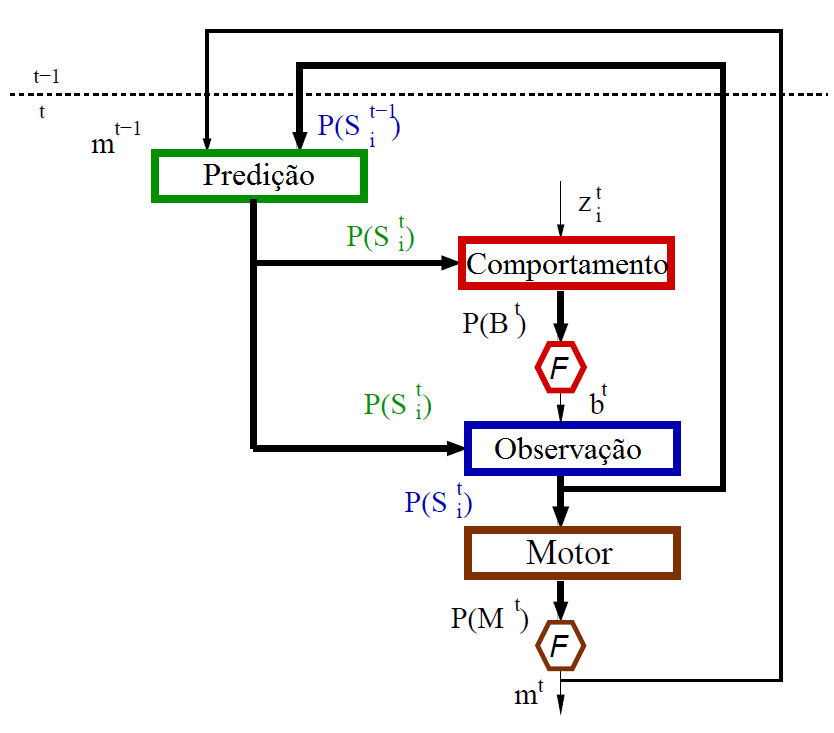
\includegraphics[width=120mm]{images/modelo_probabilistico-carla}
    \caption{\label{img:ModeloProbabilisticoCarla}Filtro Bayesiano utilizando Q Learning para Seleção de Comportamento.}
\end{figure}

Cada etapa dessa pode ser descrita como:


\subsubsection{Predição}

Nessa etapa, a partir da ação escolhida no período anterior de tempo, se faz uma estimativa de qual será o estado após sua execução.

\begin{equation}
    P \left( S^t B^t \mid z^{0: t-1} z_b^{0: t-1} m^{0: t-1} \pi_f \right) \propto \sum\limits_{S^{t-1} B^{t-1}}
        \left(
            \begin{array}{l}
                P \left( S^t \mid S^{t-1} m^{t-1} \pi_f \right) \times P \left( B^t \mid \pi_f \right) \\
                \times P \left( m^{t-1} \mid S^{t-1} B^{t-1} m^{t-2} \pi_f \right)\\
                \times P \left( S^{t-1} B^{t-1} \mid z^{0: t-1} z_b^{0: t-1} m^{0: t-2} \pi_f \right)
            \end{array}
        \right)
\end{equation}


\subsubsection{Escolha de comportamento}

Essa etapa é onde a escolha do comportamento acontece. Primeiro se calcula a função à seguir para cada comportamento $ z_b \in Z_b^t $ e para o conjunto de probabilidades $ a^t \in A^t $ de se encontrar em cada estado.

\begin{equation}
    	Q \left( a^t, Z_b^t \right) = \omega^1 \cdot f^1 \left( a^t, Z_b^t \right) + \omega^2 \cdot f^2 \left( a^t, Z_b^t \right) + \cdots + \omega^n \cdot f^n \left( a^t, Z_b^t \right)
\end{equation}

Depois, se escolhe um comportamento a partir desses valores calculados, sendo o escolhido o que maximize essa função.

\subsubsection{Observação}

A partir dos sensores presentes no robô e do valor de $ z_b $, obtido com o algoritmo de aprendizado, se atualiza o belief state do agente.

\begin{equation}
    P \left( S^t B^t \mid z^{0: t} z_b^{0: t} m^{0: t-1} \pi_f \right) \propto
        \left(
            \begin{array}{l}
                P \left( z^t \mid S^t \pi_f \right) \times P \left( z_b^t \mid B^t \pi_f \right) \\
                \times P \left( S^t B^t \mid z^{0: t-1} z_b^{0: t-1} m^{0: t-1} \pi_f \right)
            \end{array}
        \right)
\end{equation}


\subsubsection{Escolha de ação motor}

Por último se faz a seleção de uma ação a ser executada pelo robô. Para isso, calcula-se as probabilidade de se executar cada ação e se escolhe a com maior valor.
		
\begin{equation}
    P \left( M^t \mid z^{0: t} z_b^{0: t} m^{0: t-1} \pi_f \right) \propto \sum\limits_{S_i^{t-1} B^{t-1}}
        \left(
            \begin{array}{l}
                P \left( M^t \mid S^t B^t m^{t-1} \pi_f \right)\\
                \times P \left( S^t B^t \mid z^{0: t} z_b^{0: t} m^{0: t-1} \pi_f \right)
            \end{array}
        \right)
\end{equation}


\section{Ambiente de testes e simulação}

